\section{Optimization of Systems Using
Preferences}\label{sec:completed_pref_opt}

\emph{Material in this section based on
\citet{thatte2017sample} (in review) \cite{thatte2017sample}} 
\linebreak
 
As discussed in \cref{sec:back_optimization} previous work has explored learning
from qualitative feedback such as preferences in order to circumvent defining
objective functions and using Bayesian optimization in order to reduce the
number of experiments requried to optimize a system. In this section, we present
a new optimization algorithm, Predictive Entropy Search with Preferences
(PES-P), that combines these two ideas. The algorithm uses preference queries
between pairs of control parameters to avoid the a priori definition of features
and to consider unquantifiable qualities of the desired behavior. The algorithm
further incorporates black-box Bayesian optimization to ensure its preference
queries gather information efficiently without relying on a system model.

In developing the algorithm, we make three main contributions. First, we adapt
an acquisition function previously proposed for interval scale feedback to the
preference feedback case. This acquisition function seeks a pair of parameters
for which a preference will maximally reduce the entropy of the distribution of
objective function optima. Second, we compare in simulation the performance of
the proposed optimization method against the expected improvement method (EI)
and uniform random sampling via Latin hypercubes (LH) for two classes of
examples: optimizing randomly generated objective functions and tuning the
control parameters of simulated dynamical systems.  Finally, we compare the
performance of the three methods for the task of optimizing the control
parameters of a robotic prosthesis given real user feedback.

\subsection{Preliminaries} 
\subsubsection{Learning from Preferences}

To learn latent objective functions from preferences, we rely on the method
developed by \citeauthor{chu2005preference}~\citep{chu2005preference}, briefly
reviewed here.  The method considers a training dataset $D_n$ of $n$ preferences
between pairs of points, $\{x_1^\tn{a} \succ x_1^\tn{b}, \ldots, x_k^\tn{a}
\succ x_k^\tn{b}, \ldots, x_n^\tn{a} \succ x_n^\tn{b}\}$. These points can, for
instance, represent control policy parameters. From the dataset, the method
finds a posterior distribution of latent objective functions $\vecf{f}$,
\begin{align}
    \prob{\vecf{f}|D_n} = \frac{\prob{D_n|\vecf{f}}
        \prob{\vecf{f}}}{\prob{D_n}}.
    \label{eq:bayes_rule}
\end{align}
where $\vecf{f} = [f(x_1^\tn{a}), f(x_1^\tn{b}), \ldots, f(x_n^\tn{a}),
f(x_n^\tn{b})]^T$. First, the method assumes that the prior distribution of
objective functions is a zero-mean \emph{Gaussian process} (GP),
$\prob{\vecf{f}} = \mathcal{N}(0, \Sigma)$. An appropriate kernel, $\Sigma_{i,j}
= \func{k}(x_i,x_j)$, describes the elements of the covariance matrix $\Sigma$.
(See~\citep{williams2006gaussian} for a full description of GPs.) Second,
$\prob{D_n|\vecf{f}}$ is the overall likelihood of preferences in the
dataset given specific reward function values and is modeled as the product of
the likelihood of each independent preference in the dataset,
\begin{align}
    \prob{D_n|\vecf{f}} &= \prod_{k=1}^n \prob{x_k^\tn{a} \succ x_k^\tn{b} 
            | f(x_k^\tn{a}), f(x_k^\tn{b})} 
        = \prod_{k=1}^n \Phi(q_k),
    \label{eq:likelihood}
\end{align}
where $\prob{x_k^\tn{a} \succ x_k^\tn{b} | f(x_k^\tn{a}), f(x_k^\tn{b})}$ is the
probability of a preference if Gaussian noise with variance $\sigma^2$ corrupts
the function values, $\Phi(\cdot)$ is the cumulative distribution function of a
normal distribution, and $q_k = \frac{f(x_k^\tn{a}) - f(x_k^\tn{b})}{\sqrt{2}
\sigma}$.  In essence, the likelihood model increases the certainty of a
preference between $x_k^\tn{a}$ and $x_k^\tn{b}$ as the difference between
$f(x_k^\tn{a})$ and $f(x_k^\tn{b})$ widens. 

To obtain the posterior distribution $\prob{\vecf{f}|D_n}$ the method
approximates \cref{eq:bayes_rule} with a Gaussian distribution. As a result, the
predictive distribution (subscript p) of the objective function at test points,
$\vecf{f}[\tn{t}]$, is also Gaussian, $\prob{\vecf{f}[\tn{t}] | D_n} =
\mathcal{N} \left( \mu_\tn{p}, \Sigma_\tn{p} \right)$. Finally, the predictive
distribution of a preference between two points $x^\tn{a}$ and $x^\tn{b}$ is 
\begin{align} 
    \prob{x^\tn{a} \succ x^\tn{b} |D_n} 
    &=\hspace{-2pt}\int \prob{x^\tn{a} \succ x^\tn{b}|\vecf{f}[\tn{t}],D_n}
    \prob{\vecf{f}[\tn{t}]| D_n} \tn{d} \vecf{f}[\tn{t}] 
        \label{eq:prob_of_pref}\\
    &= \Phi \left(\frac{\mu^\tn{a} - \mu^\tn{b}}{\sigma_\tn{p}} \right),
        \label{eq:p_pref} \\ 
    \sigma_\tn{p}^2 &= 2\sigma^2 + \Sigma_\tn{p}^\tn{aa} + \Sigma_\tn{p}^\tn{bb}
        - \Sigma_\tn{p}^\tn{ab} - \Sigma_\tn{p}^\tn{ba}.
\end{align}

\Cref{fig:pes_plot}a provides an example of how the method estimates a
ground-truth objective function shown in purple. The blue line and shaded area show
the mean and standard deviation of the posterior distribution of objective
functions, $\prob{\vecf{f}_\tn{t}|D_n}$, after two preference queries between
pairs of parameters (orange, higher is preferred over lower value). The queries
have the effect of lifting the estimated objective function close to preferred
points and pushing it down close to unpreferred points, approximating the true
objective function over time.

\subsubsection{Active Learning for Optimization}
Learning from preferences describes how to find a distribution of objective
functions given a dataset of comparisons. The question now becomes how to
efficiently solicit preferences from the user. As our main goal is to find the
optimal parameters $x^*$, we should forgo modeling the objective function
accurately in all parameter regions and instead focus on regions where the
objective might be high. Bayesian optimization addresses this problem with an
acquisition function that helps to efficiently sample training data.
\begin{marginfigure}
    \centering
    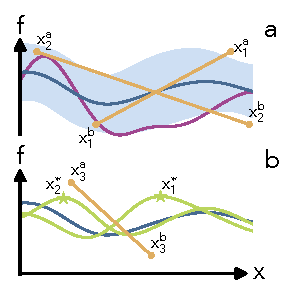
\includegraphics[width=\linewidth]{pes_plot}
    \caption{Learning from preferences. (a) Mean and standard deviation of
    $\prob{\vecf{f}[\tn{t}]|D_n}$ (blue) after two preferences queries (orange)
    from the true objective function (purple). (b) Mean of
    $\prob{\vecf{f}[\tn{t}]|D_n}$ (blue) and means of
    $\prob{\vecf{f}[\tn{t}]|D_n, x_m^*}$ (green) for two samples of $x_m^*$.
    PES-P queries a new comparison (orange) for which the preference is
    currently uncertain, but on average is certain after conditioning on all
    $x_m^*$.}\label{fig:pes_plot}
\end{marginfigure}

One such acquisition function is the expected improvement, which has been used
both in the context of preference feedback~\citep{eric2008active} and interval
scale feedback~\citep{jones1998efficient},
\begin{equation}
    \func{EI}{x} = (\mu^* - \mu(x))\Phi(d) + s(x)\phi(d),
    \label{eq:expected_improvement}
\end{equation}
where $d = (\mu^* - \mu(x))/s(x)$, $\mu^*$ is the mean of the current estimate
of the optimum, and $\mu(x)$ and $s(x)$ are the mean and standard deviation of
the objective of a new point $x$, respectively. As an alternative, for interval
scale feedback,~\citep{hennig2012entropy} and~\citep{hernandez2014predictive}
proposed acquisition functions that seek to reduce the uncertainty in the
distribution of objective function optima, measured in terms of the differential
entropy. For example, the Predictive Entropy Search acquisition
function~\citep{hernandez2014predictive} seeks a point $x$ that is expected to
reduce the entropy of the distribution of optima $x^*$ after observing its value
$y$,
\begin{align}
    \alpha_n \left(x \right) = \funcsb{H}{\prob{x^*|D_n}} 
        - \funcsb{E}[\prob{y|x, D_n}]{\funcsb{H}{\prob{x^*|y, x, D_n}}},
    \label{eq:pes_interval_scale}
\end{align}
where $\funcsb{H}{\prob{x}} = - \int \prob{x} \log \prob{x} \tn{d} x$
is the differential entropy. The authors of these methods have shown they can
outperform EI\@. 

% -------
% Methods
% -------
\subsection{Methods}
Our goal is to simultaneously address both the difficulty of defining objective
functions when an expert cannot demonstrate the desired robot behavior and the
expense of running experiments on hardware. To this end, we adapt the Predictive
Entropy Search acquisition function (\cref{eq:pes_interval_scale}) to the
preference learning case.

\subsubsection{Acquisition Function}
To obtain the optimal parameters $x^*$ with the smallest number of preference
queries, we solicit preferences that maximize the expected information gain
about the distribution of objective function optima $\mathrm{P}(x^*|D_n)$.
Adapting \cref{eq:pes_interval_scale} to preference feedback yields
\begin{fullwidth}
\begin{align}
    &\alpha_n \left(x^\tn{a}, x^\tn{b}\right) 
        = \funcsb{H}{\prob{x^*|D_n}} - \funcsb{E}[\prob{y|x^\tn{a},x^\tn{b},D_n}]
            {\funcsb{H}{\prob{x^*|y, x^\tn{a}, x^\tn{b}, D_n}}},
    \label{eq:acquisition_orig}
\end{align}
\end{fullwidth}
where $y$ is a binary random variable that represents the preference between
$x^\tn{a}$ and $x^\tn{b}$. The first term in this function is the current
entropy of objective function optima and the second term is the entropy of
optima after observing the preference $y$. As we have not yet observed the
preference, we take the second term in expectation over the two possible
preference outcomes.

As discussed in~\citep{hernandez2014predictive}, this acquisition function is
intractable to compute. However, following the approach used for the original
PES algorithm, we can rewrite~\cref{eq:acquisition_orig} in terms of the
entropies of the predictive distribution of the preference between $x^\tn{a}$
and $x^\tn{b}$,
\begin{fullwidth}
\begin{align}
    \alpha_n \left(x^\tn{a}, x^\tn{b} \right) &= 
        \funcsb{H}{\prob{y|x^\tn{a}, x^\tn{b}, D_n}}
            - \funcsb{E}[\prob{x^*|D_n}]{\funcsb{H}
            {\prob{y| x^*, x^\tn{a}, x^\tn{b}, D_n}}} \\
        &\approx \funcsb{H}{\prob{y|x^\tn{a}, x^\tn{b}, D_n}}
            - \frac{1}{M} \sum_{x_m^* \sim {\prob{x_m^*|D_n}}}^M 
            \hspace{-0.03in}\funcsb{H}{\prob{y| x_m^*, x^\tn{a},x^\tn{b},D_n}}.
        \label{eq:aq_approx}
\end{align}
\end{fullwidth}
This reformulation significantly improves computability. First, the new
acquisition function uses the entropies of probabilities of preferences, given
by~\cref{eq:p_pref}. Second, we now take the expectation over $\prob{x^*|D_n}$,
which we can perform by sampling $M$ functions from
$\prob{\vecf{f}[\tn{t}]|D_n}$ and optimizing each one to get $M$ samples of
$x^*$ (see Appendix for details). Finally, the second term no longer requires
conditioning the GP on every pair of $x^\tn{a}$ and $x^\tn{b}$ considered during
optimization of the acquisition function.  Instead, we only have to condition
the Gaussian process $M$ times on $(x_m^*, D_n)$.

For the experiments in~\cref{s:results} we choose $M = 12$, which allows us to
construct and optimize $\alpha_n(x^\tn{a}, x^\tn{b})$ in about five seconds,
which is fast enough for our prosthesis application. Although 12 samples of
$x^*$ is not enough to compute an accurate expectation over $\prob{x^*|D_n}$,
interpreting the algorithm as an example of active learning by disagreement may
explain why it still works well.  As shown in~\cref{fig:pes_plot}b, optimizing
the acquisition function chooses a pair $x^\tn{a}$ and $x^\tn{b}$ for which the
preference is currently uncertain, but certain on average after conditioning on
all $x_m^*$. The sampled $x_m^*$ do not necessarily agree on which point is
preferred; hence, after observing the preference, the algorithm can rule out
$x_m^*$ that made the model certain but wrong about the preference. This
intuition is similar to that provided by \citep{houlsby2012collaborative} for
Bayesian active learning by disagreement for GP classifiers.

\subsubsection[Conditioning the Gaussian Process on optima]{Conditioning the
Gaussian Process on $x^*$} The second term on the right side
of~\cref{eq:aq_approx} requires us to compute the distribution of the
preference given the location of the optimum,
\begin{fullwidth}
\begin{align}
&\prob{y| x_m^*, x^\tn{a}, x^\tn{b}, D_n} =
    \int \prob{x^\tn{a} \succ x^\tn{b} | \vecf{f}[\tn{t}], x_m^*, D_n} 
    \prob{\vecf{f}[\tn{t}] | x_m^*, D_n} \tn{d} \vecf{f}[\tn{t}].
    \label{eq:predic_pref_w_constraint}
\end{align}
\end{fullwidth}
It is not directly feasible to condition the predictive distribution on $x^*$,
so instead we turn to approximating this condition with three constraints (see
\hyperlink{sec:appendix}{appendix} for details):

C1: First we impose that $x^*$ is a local maximum by ensuring that the gradient
of $f(x^*)$ is zero and its Hessian is negative definite. We further simplify
the Hessian constraint to only require that the Hessian's off-diagonal elements
are zero and its diagonal elements are less than zero. We implement the gradient
and off-diagonal constraints by conditioning the prior, $\prob{\vecf{f}}$, on
derivative observations as outlined in~\citep{solak2003derivative}. To constrain
the diagonal elements of the Hessian, we amend the likelihood term in
\cref{eq:bayes_rule} by adding terms that penalize Hessians with positive
diagonal elements.

C2: Second, we try to ensure that $x^*$ is also a global maximum by enforcing
that $f(x^*)$ is greater than the function values of all training points sampled
so far. We impose this constraint by adding more preference relations into the
likelihood term in \cref{eq:bayes_rule} between $x^*$ and all training points.

C3: Finally, to further ensure that $f(x^*)$ is a global maximum, we require
that it is also larger than the function values of the two new test points,
$f(x^\tn{a})$ and $f(x^\tn{b})$. Whereas C2 ensures $f(x^*)$ exceeds function
values in areas explored so far, C3 ensures that $f(x^*)$ also exceeds function
values in unexplored regions. We approximate this constraint analytically by
conditioning on the single constraint $f(x^*) > (f(x^\tn{a}) + f(x^\tn{b}))/2$
using the
method detailed in~\citep{xu2010estimation}.
\begin{algorithm}[t]
    \caption{Predictive Entropy Search with Preferences}
    \begin{algorithmic}[1]
        \Procedure{PES-P}{}
            \State{$D_n = \varnothing$}
            \For{$n \gets 0$ \textbf{to} $N-1$}\Comment{$N$ iterations}
            	\State{$F \gets \{\vecf{f}[m] \sim \prob{\vecf{f}[\tn{t}]| D_n} 
                    | m \in [1, M]\}$}
               	\State{$X^* \gets \{\arg \max_x \left(\vecf{f}[m] \right) 
                    | \vecf{f}[m] \in F \}$}
                \State{$(x_{n+1}^\tn{a}, x_{n+1}^\tn{b}) \gets \arg
                    \max_{(x^\tn{a}, x^\tn{b})} 
                    \funcil{\alpha}[n]{x^\tn{a},x^\tn{b};X^*}$}
                \State{$y_{n+1} \gets 
                    \textsc{QueryUserPref}(x_{n+1}^\tn{a}, x_{n+1}^\tn{b})$}
                \State{$D_{n+1}\hspace{-0.25em}\gets\hspace{-0.25em}
                    D_n \cup (x_{n+1}^\tn{a}, x_{n+1}^\tn{b}, y_{n+1})$}
            \EndFor{}
            \State{$\textbf{return} \ x^* \gets \arg \max_x
                \func{mode}{\prob{\vecf{f}[\tn{t}](x)| D_N}}$}
        \EndProcedure{}
        \Statex{}
        \Function{$\alpha_n$}{$x^\tn{a}, x^\tn{b}; X^*$}
            \Comment{acquisition function}
            \State{$h \gets \left\{\funcsb{H}{\prob{y|x^\tn{a}, x^\tn{b}, D_n, 
                \tn{C1}, \tn{C2}, \tn{C3}}} | x_m^* \in X^* \right\}$}
            \State{$\textbf{return} \ \funcsb{H}{\prob{y|x^\tn{a},x^\tn{b},D_n}} 
                - \func{mean}{h}$}
        \EndFunction{}
    \end{algorithmic}\label{alg:pesp}
\end{algorithm}

\subsubsection{Algorithm Summary}
With constraints C1 to C3, at each iteration we can efficiently compute the
acquisition function, \cref{eq:aq_approx}. We summarize the resulting Predictive
Entropy Search with Preferences (PES-P) algorithm as follows (\cref{alg:pesp}):
At each iteration $n$, first, the algorithm samples $M$ objective functions from
the current distribution, $\prob{\vecf{f}[\tn{t}]|D_n}$, and optimizes each one
to generate $M$ samples of $x^*$ (lines 4 and 5).  Next, using the set of
sampled optimums $X^*$, we maximize the acquisition function to obtain the next
two points to present to the user $x_{n+1}^\tn{a}$ and $x_{n+1}^\tn{b}$ (lines 6
and 12--15). Note: we can precompute the effect of C1 and C2 before evaluating
$\funcil{\alpha}[n]{x^\tn{a}, x^\tn{b}}$ as these two constraints do not depend
on $x_{n+1}^\tn{a}$ and $x_{n+1}^\tn{b}$. On the other hand, C3 depends directly
on $x_{n+1}^\tn{a}$ and $x_{n+1}^\tn{b}$ and therefore is computed within the
acquisition function for every pair of points considered during the optimization
of $\funcil{\alpha}[n]{x^\tn{a}, x^\tn{b}}$. We then query the user to obtain
their preference $y_{n+1}$ between these two points and add it to the dataset of
preferences (lines 7 and 8). Finally, at the end of the $N$ iterations of the
algorithm, we return the optimum $x^*$ of the most likely function,
$\func{mode}{\prob{\vecf{f}[\tn{t}](x)| D_N}}$, which is equal to the posterior
mean function in the Gaussian process case (line 10). While it may be more
correct to return $\func{mode}{\prob{x^*|D_N}}$, we do not do this as the PES
algorithm seeks to avoid approximating this distribution.

\subsection{Results}\label{s:results}
We test the ability of PES-P to solve optimization problems in four cases with
increasing realism from the optimization of randomly generated objective
functions drawn from a GP, to the tuning of feedback gains of random linear
systems and a neuromuscular walking model, to the optimization of control
parameters for a powered transfemoral prosthesis given real user feedback. In
all four cases, we compare the performance of the proposed algorithm to the
expected improvement criterion (EI) (\cref{eq:expected_improvement}) and random
sampling via Latin hypercubes (LH)\sidenote[][2.25in]{LH sampling divides the
parameter space into ${(2N)}^D$ hypercubes, where $D$ is the dimensionality of
the space.  $2N$ samples are placed such that each hypercube has at most one
sample and there is at most one filled hypercube along any row of hypercubes
when viewed along any direction.  This method ensures that the samples are
roughly uniformly distributed in the entire space. At each iteration we choose
two of these samples to query users.}~\citep{mckay2000comparison}. For the three
simulated cases, we show results over 20 trials and measure performance in terms
of the immediate regret, defined as $IR = |f(\tilde x_n^*) - f(x^*)|$, versus
the number iterations.  Here, $f(\tilde x_n^*)$ is the objective value of the
current estimate of the optimum at this iteration, $f(x^*)$ is the value of the
true optimum, and an iteration consists of a single preference query between two
points.  Additionally, we also check the statistical significance of the
reduction in IR obtained by PES-P compared to both EI and LH via one-sided
Mann-Whitney $U$ tests $(p < 0.05)$.

\begin{figure*}[t!]
    \centering
    \begin{subfigure}[b]{0.24\textwidth}
    	\centering
        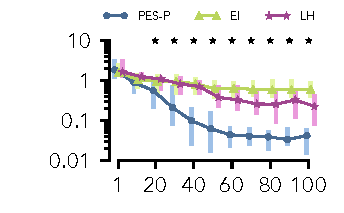
\includegraphics[width = \textwidth]{y_err2_legend}
        \vspace{-20pt}\caption{2 dimensions, $\lambda = 0.1$}\label{fig:y_err2}
    \end{subfigure}
    \begin{subfigure}[b]{0.24\textwidth}
    	\centering
        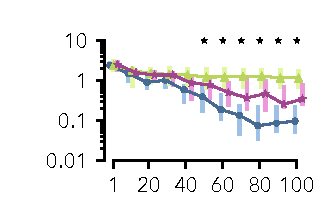
\includegraphics[width = \textwidth]{y_err3}
        \vspace{-20pt}\caption{3 dimensions, $\lambda = 0.2$}\label{fig:y_err3}
    \end{subfigure}
    \begin{subfigure}[b]{0.24\textwidth}
    	\centering
        \vspace{10pt}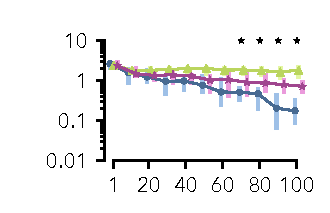
\includegraphics[width = \textwidth]{y_err4}
        \vspace{-20pt}\caption{4 dimensions, $\lambda = 0.3$}\label{fig:y_err4}
    \end{subfigure}
    \begin{subfigure}[b]{0.24\textwidth}
    	\centering
        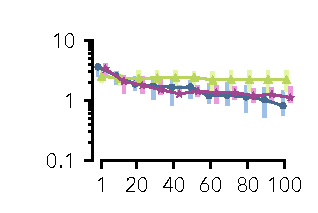
\includegraphics[width = \textwidth]{y_err5}
        \vspace{-20pt}\caption{5 dimensions, $\lambda = 0.4$}\label{fig:y_err5}
    \end{subfigure}
    \vspace{0.1in}
    \begin{subfigure}[b]{0.24\textwidth}
        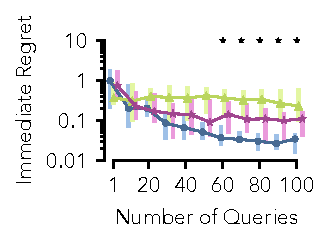
\includegraphics[width = \textwidth]{y_err3LQR}
        \vspace{-20pt}\caption{LQR 3 dim}\label{fig:LQR_3}
    \end{subfigure}
    \begin{subfigure}[b]{0.24\textwidth}
    	\centering
        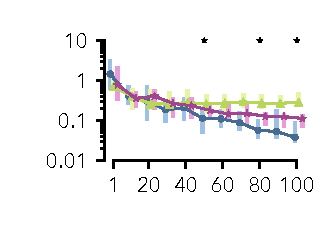
\includegraphics[width = \textwidth]{y_err4LQR}
        \vspace{-20pt}\caption{LQR 4 dim}\label{fig:LQR_4}
    \end{subfigure}
    \begin{subfigure}[b]{0.24\textwidth}
    	\centering
        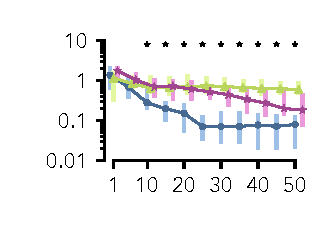
\includegraphics[width = \textwidth]{y_err2Neuro}
        \vspace{-20pt}\caption{Biped Walking  2 dim}\label{fig:Neuro_2}
    \end{subfigure}
    \begin{subfigure}[b]{0.24\textwidth}
    	\centering
        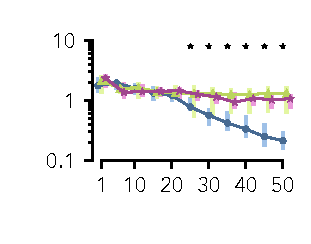
\includegraphics[width = \textwidth]{y_err3Neuro}
        \vspace{-20pt}\caption{Biped Walking 3 dim}\label{fig:Neuro_3}
    \end{subfigure}
    \caption{Performance of predictive entropy search with preferences (PES-P),
    expected improvement (EI), and Latin hypercube random sampling (LH) for
    optimizing random objective functions sampled from a GP (a-d), and tuning
    feedback control parameters of random linear systems (e-f) and a biped
    walking model (g-h). Shown are the median and interquartile range over 20
    trials of the immediate regret (IR) against the number of preference
    queries. Black stars indicate iterations for which PES-P achieves
    statistically significant stochastic reductions in IR compared to both EI
    and LH according to one-sided Mann-Whitney $U$ tests $(p <
    0.05)$.}\label{fig:y_err_sim}
\end{figure*}

\subsubsection{Optimizing Randomly Generated Objective Functions}

To avoid inducing bias by hand-engineering test functions, we first evaluate the
algorithm on random synthetic objective functions. We generate objective
functions on the domain $x \in {[-1, 1]}^D$ by sampling a vector of 500 function
values from a GP prior with a quadratic mean, $\mu(x) = - x^\tn{T} x$, and
isometric squared exponential covariance $\funcil{k}{x_i,x_j} = \exp
\left(\frac{-1}{2 \lambda} x_i^T x_j \right)$. We use a quadratic mean function
to bias the function distribution away from those that have their optimum on a
boundary of the domain, as these functions are easier to optimize. We continue
to generate the rest of the function as it is optimized by conditioning the GP
on the 500 seed values and all function values sampled during the optimization.
We assume the mean of the final function distribution is the true objective
function. To simulate more realistic situations, we provide the algorithms with
noisy preferences from the sampled function values ($\sigma^2 = 0.1$).

Figures~\ref{fig:y_err_sim}a-d show the immediate regret for two to five
dimensional problems with $\lambda$, the length scale of the kernel, scaling
from 0.1 to 0.4 as the dimensionality of the problem increases. On two to four
dimensional problems, PES-P outperforms EI and LH by achieving statistically
significant reductions in IR\@. However, as the dimensionality increases, it
takes more iterations for this advantage to become apparent. In the five
dimensional case, there is no significant difference between PES-P and LH,
likely due to $M=12$ samples of $x_m^*$ being insufficient and the difficulty of
accurately sampling $x_m^*$ in higher dimensions.

\subsubsection{Tuning Controllers for Random Linear Systems}
Next, we test the ability of PES-P to optimize simple control systems by
optimizing the feedback gains $K$ for $D$-dimensional single-input linear
systems $\dot{\xi} = A \xi + Bu$ with feedback $u = K \xi$. We sample the
elements of the $A$ matrix from the standard normal distribution while $B =
{[0_{1 \times (D-1)}, 1]}^\tn{T}$. We assume a quadratic instantaneous cost
resulting in the objective function
\begin{equation}
    f(K) = - \int_0^{t_f} \xi_K^\tn{T}(t) (Q + K^T R K) \xi_K(t) dt,
\end{equation}
where $\xi_K(t)$ is the evolution of the state under the control policy $K$ and
a fixed initial condition $\xi_0$, $Q = I_{D \times D}$ and $R = 1$. To obtain a
finite search domain, we find the stable range of parameters by varying the
elements of the true optimal control parameters $K^*$ one at a time while
keeping other elements constant. We scale and shift this region to map to the
domain ${[-1, 1]}^D$. Finally, we use the Automatic Relevance Determination
Gaussian Kernel and optimize the hyperparameters at each iteration by maximizing
the posterior probability of the hyperparameters under a gamma
hyperprior~\citep{chu2005preference,
williams2006gaussian}. In order to apply a consistent noisy preference model
$(\sigma^2 = 0.1)$ across all sampled systems, we transform all objective values
by first mapping them through $-\log(-f(K))$ and then shifting and scaling the
values by the mean and range of the values of $10^D$ randomly sampled
controllers. 

Figures~\ref{fig:y_err_sim}e and~\ref{fig:y_err_sim}f show the resulting
optimization performance on three and four dimensional systems. In the 3
dimensional case, PES-P achieves a lower median IR than LH after 30 iterations.
This difference becomes significant after 60 iterations. In the 4 dimensional
case, PES-P significantly outperforms LH after 50 iterations, but the
significance of this improvement is sporadic as the iterations continue. A
possible reason for the reduced performance difference between PES-P and LH in
the LQR problem as compared to the random objective function problems is the
existence of hard-to-optimize flat regions in the LQR objective functions. This
suggests that PES-P may be more well suited for problems that have clear
optimum.
\subsubsection{Tuning Control Parameters of a Walking Model
    }\label{sec:sim_neuro}
In the third case, we test the ability of PES-P to optimize the feedback gains
for a neuromuscular model of walking~\citep{thatte2016toward}, a system with a
complex non-linear controller addressing the specific application domain of
human locomotion. We perform two and three dimensional optimizations, in which
we tune the feedback gains for a subset of the model's muscle actuators.  We use
the negative cost of transport plus the distance walked over a 20 second time
span as the objective function. As in the previous linear systems example, we
obtain noisy preferences between parameters and optimize the hyperparameters at
every iteration.

Figures~\ref{fig:y_err_sim}g and~\ref{fig:y_err_sim}h show the performance of
PES-P, EI, and LH\@. In this example, PES-P achieves a significant reduction in
IR in just 10 iterations in the 2-dimensional case and in 25 iterations in the 3
dimensional case.  Furthermore, in the 3D case the PES-P's median solution is
approximately 10 times better than those found by EI or LH\@. 

\subsubsection{Tuning a Transfemoral Prosthesis from User Preferences} 
\begin{figure*}[t]
    \centering
    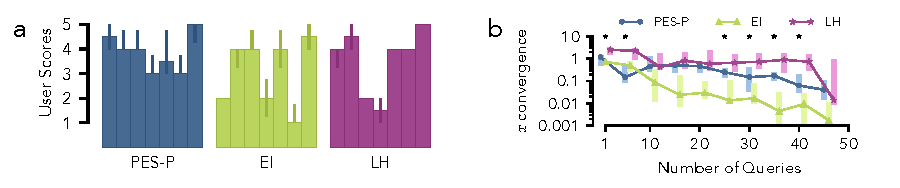
\includegraphics[width=\textwidth]{prosthesis_result_combined.pdf}
    \caption{Optimization of prosthesis control with user preferences. (a)
    Median and interquartile range of user scores achieved by PES-P, EI and LH
    after 50 iterations (total of 42 scores per algorithm: seven users times six
    scorings). (b) Median and interquartile range of convergence achieved by the
    three algorithms as measured by the Euclidean distance between the current
    and final estimates of the optimum. PES-P and LH achieve the same median
    score of 4 across all users but PES-P converges faster and more
    consistently. EI converges fastest but to a lower median score of
    3.}\label{fig:prosthesis_result}
\end{figure*}


In the last test case, we applied the three algorithms to optimize the control
parameters for a powered transfemoral prosthesis given real user preferences.
Specifically, a neuromuscular model similar to the one used
in~\cref{sec:sim_neuro} controls the prosthesis and we optimize the strengths
of three virtual knee muscles of this control~\citep{thatte2016toward}. 

We performed this test in a pilot study with seven healthy users. They walked
on a treadmill and wore the powered prosthesis with a modified knee brace
(compare~\citep{thatte2016toward}). We allowed all users an hour-long session to
acclimate to the device, during which they experienced a variety of controller
conditions. On a second day, we optimized the prosthesis parameters using the
three algorithms (PES-P, EI, and LH) in a random order, for 50 iterations each.
During an iteration, the users walked with two parameter settings chosen by the
algorithm (each for 10 seconds) and then indicated which setting they
preferred. After completing the three optimizations, the users walked with the
optimum parameters identified by each algorithm (in a random order) for fifteen
seconds and then rated each optimum on a 1 (bad) to 5 (good) scale. We repeated
the scoring procedure six times to cover all possible orderings of the three
optima.

\Cref{fig:prosthesis_result} summarizes the results from the optimizations with
user preferences. PES-P and LH achieved median user scores of 4 while EI
achieved a median score of 3 (Fig.~\ref{fig:prosthesis_result}a). In addition,
PES-P, LH, and EI achieved mean scores of 4.0, 3.5, and 3.1, respectively (not
shown). The gap between the mean and median scores for LH implies that LH does
not achieve high scores as consistently as PES-P. A second observation is that
PES-P converged faster than LH to the optimum as measured by the distance
between its current and final estimates, $\lVert \tilde{x}_n^* - \tilde{x}_N^*
\rVert$ (Fig.~\ref{fig:prosthesis_result}b).  Meanwhile, EI tended to converge
fastest, but to lower scoring parameters on average
(Fig.~\ref{fig:prosthesis_result}a).

\subsection{Discussion and Conclusion}\label{sec:tuning_discussion}
We presented a new optimization algorithm (PES-P) that extends Predictive
Entropy Search to preference feedback. The algorithm addresses two key problems
frequently encountered in system optimization. First, it circumvents the often
difficult process of parameterizing and learning an objective function by
directly querying users for preferences between pairs of parameters. Second, the
algorithm minimizes the required number of hardware experiments by employing
Bayesian optimization techniques that ensure the queries maximize the
information gained about the location of the optimum. Moreover, unlike previous
approaches for preference learning on robotic systems~\citep{wilson2012bayesian,
jain2013learning}, PES-P does not require a model of the system.

Our experiments show that the proposed algorithm outperforms baseline
algorithms. In most of the simulation experiments PES-P found optima that
achieved higher objective values than those found by the expected improvement
method (EI) or by random comparisons via Latin hypercubes (LH)
(\cref{fig:y_err_sim}). In the prosthesis experiment, PES-P outperformed EI and
achieved final scores similar to LH with faster convergence
(\cref{fig:prosthesis_result}). These results suggest the proposed algorithm can
help engineers optimize some types of human-in-the-loop robotic systems more
accurately, efficiently, and consistently. 

The reason why PES-P outperformed EI is likely due to the former's explicit
consideration of how the limited, noisy information obtained from a preference
query will affect the knowledge about potential objective function optima. The
acquisition function (\cref{eq:acquisition_orig}) recognizes that preferences
become more uncertain the closer two sample points are to each other. EI, on the
other hand, does not reason about noisy preferences and, instead, still assumes
it can sample values (\cref{eq:expected_improvement}). Consequently, EI ignores
the distance between sample points, which often leads to a greedy strategy that
solicits preferences between adjacent points. While this strategy can resemble
gradient ascent with convergence to local optima in a noise-free optimization,
it often failed in our simulated and real experiments characterized by noisy
observations. Note, however, that such limitations were not observed by Brochu
and colleagues~\citep{eric2008active}, who successfully used EI with preferences
to optimize parameters for a graphics application, possibly because the
associated visual task produced less noisy responses than did our simulations or
prosthesis walking task. 

Several modifications could improve the PES-P algorithm. First, using a non-zero
prior mean function governed by a set of hyperparameters could embed specific
knowledge about the problem to speed up optimization. To improve efficiency in
this way, \citep{brochu2010bayesian} details an approach for learning
hyperpriors that could be integrated with PES-P.  Second, integrating more
varied user feedback may also help improve the algorithm. For example, ``I don't
know'' responses could imply that the function values at two points are similar,
absolute good and bad ratings could encourage the algorithm to more quickly
explore promising control polices and avoid bad ones, derivative observations
could indicate the user prefers more or less of a parameter, and better than all
seen so far feedback could more clearly identify optimal parameters. Third, when
asking users to compare the optima achieved by the three algorithms, we had them
walk with each parameter set for 15 seconds and then give a rating for all
three. Subjects seemed able to recall and compare the performance of all three
parameter sets with ease. Therefore, moving forward, we should use comparisons
between three optima instead of pairwise comparisons as it will provide more
data per unit of time. Fourth, a greedier selection strategy may help improve
the performance of the algorithm in practice, as it will more quickly identify
good parameters even if they are suboptimal. With these four changes, the
algorithm may be able to tackle higher dimensional problems. Finally, we should
investigate is including time as a dimension in the GP to account for user
adaptation to the robotic system. This may allow us to eliminate the hour-long
adaptation session on the first day of our study. 

\hypertarget{sec:appendix}{\section*{Appendix}}

To obtain $X^*$ (line 5,~\cref{alg:pesp}), we sample $M$ functions from the
posterior by approximating $\prob{\vecf{f}[\tn{t}]|D_n}$ using Bayesian linear
regression with Fourier features (as outlined in~\citep{hernandez2014predictive})
and sampling $M$ feature weight vectors. As the Fourier features have analytic
derivatives, we can optimize each linear function using a second order method
with multiple restarts.

We approximate conditioning the predictive distribution on $x^*$ via three
constraints: 
\begin{description} 
    \item[C1] $x^*$ is a local maximum. $\nabla f|_{x^*} = 0$ and the
    Hessian of the objective function is negative definite by imposing
    $\func{diag}{\nabla \nabla f|_{x^*}} < 0$ and $\func{upper}{\nabla
    \nabla f|_{x^*}} = 0$. We group $\nabla f|_{x^*} = 0$ and
    $\func{upper}{\nabla \nabla f|_{x^*}} = 0$ into constraint C1.1 and
    $\func{diag}{\nabla \nabla f|_{x^*}} < 0$ into constraint C1.2.

    \item[C2] $x^*$ is preferred to current training points, $f(x^*) >
    f(x_k^\tn{a}) \textrm{ and }  f(x^*) > f(x_k^\tn{b}), \ \forall k \in [1,
    n]$.

    \item[C3] $x^*$ is preferred to new training points, $f(x^*) >
    f(x_{n+1}^\tn{a})$ and $f(x^*) > f(x_{n+1}^\tn{b})$.  
\end{description}

We precompute the effects of contraints C1 and C2 before evaluation of
$\funcil{\alpha}[n]{x^\tn{a}, x^\tn{b}}$. To impose C1 and C2, we first divide
their components into two groups: $\vecf{c} = [\nabla f|_{x^*}^\tn{T}, \
\func{upper}{\nabla \nabla f|_{x^*}}^\tn{T}]^\tn{T}$ and $\vecf{f}' =
[\vecf{f}^\tn{T},\ \func{diag}{\nabla \nabla f|_{x^*}}^\tn{T},\
f(x^*)]^\tn{T}$. Note $\tn{C1.1} \implies \vecf{c} = 0$. We write the predictive
distribution of the objective function at test points $\vecf{f}[\tn{t}]$ given
constraints C1 and C2 as
\begin{align}
    \prob{\vecf{f}[\tn{t}]|D_n, \tn{C1},\tn{C2}} = 
    \int\prob{\vecf{f}[\tn{t}]| \vecf{f}', \tn{C1.1}}  
    \prob{\vecf{f}' | D_n, \tn{C1}, \tn{C2}} \tn{d}\vecf{f}'.
    \label{eq:predictive_w_constraints}
\end{align}
We use Bayes rule to evaluate the second term in the integral, $\prob{\vecf{f}'
| D_n, \tn{C1}, \tn{C2}} = \frac{\prob{D_n , \tn{C1.2}, \tn{C2} |\vecf{f}'}
\prob{\vecf{f}'| \tn{C1.1}}}{\prob{D_n, \tn{C1.2}, \tn{C2} | \tn{C1.1}}}$. We
form the prior term $\prob{\vecf{f}'|\tn{C1.1}}$ by conditioning the joint
distribution, $\prob{\vecf{c}, \vecf{f}'}$  on $\tn{C1.1}$ given by $\vecf{c} =
0$. $\prob{\vecf{f}'|\vecf{c}} = \mathcal{N}\left( \vecf{f}'|
\Sigma_\tn{cf'}^\tn{T} \Sigma_\tn{cc}^{-1} \vecf{c}, \Sigma_\tn{f'f'} -
\Sigma_\tn{cf'}^\tn{T} \Sigma_\tn{cc}^{-1} \Sigma_\tn{cf'} \right)$ implies
$\prob{\vecf{f}'|\vecf{c}=0} = \mathcal{N}(\vecf{f}'| 0, \Sigma_\tn{f'|c})$.

We implement the likelihood term by adding extra factors to the likelihood
in~\cref{eq:bayes_rule} that impose soft constraints representing C1.2 and C2.
For C1.2 we use the penalty term $\prob{[\nabla \nabla f|_{x^*}]_{dd} <
0 | \nabla \nabla f|_{x^*}} = \Phi(-[\nabla \nabla
f|_{x^*}]_{dd}/\sigma_\tn{h})$ and for C2 we add more preference relations
between $x^*$ and all training points. 
\begin{fullwidth}
\begin{align}
    \prob{D_n, \tn{C1.2}, \tn{C2}, |\vecf{f}'} 
        &=\left[ \prod_{k=1}^n \prob{x_k^\tn{a} \succ x_k^\tn{b} 
            | f(x_k^\tn{a}), f(x_k^\tn{b})} 
        \prob{x^* \succ x_k^\tn{a} | f(x^*), f(x_k^\tn{a})} 
        \prob{x^* \succ x_k^\tn{b} | f(x^*), f(x_k^\tn{b})} \right] \notag\\
        &\quad \times  \prod_{d=1}^D \prob{{[\nabla \nabla f|_{x^*}]}_{dd} < 0
            | {[\nabla \nabla f|_{x^*}]}_{dd}} \notag \\
        &= \left[ \prod_{k=1}^n \Phi(q_k) \Phi(q_k^{\tn{a}*}) 
                \Phi(q_k^{\tn{b}*}) \right]
            \prod_{d=1}^D \Phi(q_d^\tn{h})
\end{align}
\end{fullwidth}
Where $q_k^{\tn{a}*} = \frac{f(x^*) - f(x_k^\tn{a})}{\sqrt{2} \sigma}$ and
$q_k^{\tn{b}*} = \frac{f(x^*) - f(x_k^\tn{b})}{\sqrt{2} \sigma}$ and $q_d^{h} =
\frac{-[\nabla \nabla f|_{x^*}]_{dd}}{\sigma_h}$. We use Laplace's approximation
to approximate $\prob{\vecf{f}' | D_n, \tn{C1}, \tn{C2}}$ as Gaussian,
\begin{align}
    \prob{\vecf{f}' | D_n, \tn{C1}, \tn{C2}} \approx \mathcal{N}\left(\vecf{f}'|
        \vecf{f}'_{\tn{MAP}}, {\left(\Sigma_\tn{f'|c}^{-1} +
        \Lambda_{f'_\tn{MAP}} \right)}^{-1} \right),
    \label{eq:rprime_given_constraints}
\end{align}
where $\vecf{f}'_\tn{MAP} = \arg \min_{\vecf{f}'} -\log
\prob{\vecf{f}' | D_n, \tn{C1}, \tn{C2}}$ and $\Lambda_\tn{f'_{MAP}}$ is the
Hessian of $-\log \prob{D_n , \tn{C1.2}, \tn{C2}|\vecf{f}'}$ evaluated at
$\vecf{f}'_\tn{MAP}$.

We compute the first term in~\cref{eq:predictive_w_constraints},
$\prob{\vecf{f}[\tn{t}]|\vecf{f}', \tn{C1.1}}$ by conditioning the joint
distribution $\prob{\vecf{c}, \vecf{f}', \vecf{f}[\tn{t}]}$
on $\vecf{f}'$ and $\vecf{c} = 0$,
\begin{fullwidth}
\begin{align}
    \prob{\vecf{f}[\tn{t}] | \vecf{f}', \vecf{c}=0} = \mathcal{N} \left(
        \vecf{f}[\tn{t}] | 
        \left( \Sigma_\tn{ct}^\tn{T} B + \Sigma_\tn{f't}^\tn{T} D \right) 
            \vecf{f}', \Sigma_\tn{tt} - 
        \begin{bmatrix} 
            \Sigma_\tn{ct}^\tn{T} & \Sigma_\tn{f't}^\tn{T} 
        \end{bmatrix}
        \begin{bmatrix}
            A & B \\ C & D
        \end{bmatrix}
        \begin{bmatrix} \Sigma_\tn{ct} \\ \Sigma_\tn{f't} \end{bmatrix} \right),
        \label{eq:P_r_given_rprimec}
\end{align}
\end{fullwidth}
where,
    $\begin{bmatrix}
        A & B \\ C & D
    \end{bmatrix} = 
    \begin{bmatrix}
        \Sigma_\tn{cc} & \Sigma_\tn{cf'} \\ \Sigma_\tn{cf'}^\tn{T} &
        \Sigma_\tn{f'f'}
    \end{bmatrix}^{-1}$.
We can substitute~\cref{eq:P_r_given_rprimec}
and~\cref{eq:rprime_given_constraints} into~\cref{eq:predictive_w_constraints}
to yield the predictive distribution subject to constraints $C1$ and $C2$.
\begin{fullwidth}
\begin{align}
    \prob{\vecf{f}[\tn{t}]|D_n, \tn{C1}, \tn{C2}} = &\mathcal{N}
        \left( \vecf{f}[\tn{t}] | 
    (\Sigma_\tn{ct}^\tn{T} B + \Sigma_\tn{f't}^\tn{T} D) 
        \vecf{f}'_\tn{MAP}, \Sigma_\tn{tt} - 
        \begin{bmatrix} 
            \Sigma_\tn{ct}^\tn{T} & \Sigma_\tn{f't}^\tn{T} 
        \end{bmatrix}
        \begin{bmatrix}
            A & B \\ C & D
        \end{bmatrix}
        \begin{bmatrix} 
            \Sigma_\tn{ct} \\ \Sigma_\tn{f't} 
        \end{bmatrix} \right. \notag \\
        & \left. + \left( 
            \Sigma_\tn{ct}^\tn{T} B + \Sigma_\tn{f't}^\tn{T} D\right)
        {\left(\Sigma_\tn{f'|c}^{-1} + \Lambda_\tn{f'_{MAP}}\right)}^{-1}
        {\left(\Sigma_\tn{ct}^\tn{T} B + \Sigma_\tn{f't}^\tn{T} D
        \right)}^\tn{T} \right).
    \label{eq:pred_dist_constrain_xstar}
\end{align}
\end{fullwidth}
We obtain $\prob{\vecf{f}[\tn{t}]|D_n, \tn{C1}, \tn{C2}, \tn{C3}}$ by
analytically conditioning \cref{eq:pred_dist_constrain_xstar} on the single
inequality $f(x_m^*) > (f(x^\tn{a}) + f(x^\tn{b}))/2$ using the method detailed
in~\citep{xu2010estimation}. Finally, using~\cref{eq:predic_pref_w_constraint} we
can compute the predictive distributions of preferences given the locations of
$x_m^*$.

To optimize $\funcil{\alpha}[n]{x^\tn{a}, x^\tn{b}}$ (line 7,~\cref{alg:pesp})
we construct its gradient by evaluating $\prob{\vecf{f}[\tn{t}] | D_n}$ and
$\prob{\vecf{f}[\tn{t}] | D_n, \tn{C1},\tn{C2},\tn{C3}}$ at test points
$x^\tn{a}$ and $x^\tn{b}$ as well as points offset by $\delta_x = \pm 0.001$
along each dimension. We then optimize $\alpha_n(x^\tn{a}, x^\tn{b})$ via
gradient ascent.
